% CT6027 Academic Journal Paper Template
% !TEX program = pdflatex
\documentclass[11pt,a4paper]{article}

\usepackage[a4paper,margin=1in]{geometry}
\usepackage[T1]{fontenc}
\usepackage[utf8]{inputenc}
\usepackage{lmodern}
\usepackage{microtype}
\usepackage{graphicx}
\usepackage{booktabs}
\usepackage{caption}
\usepackage{hyperref}
\usepackage[nameinlink]{cleveref}
\usepackage{tikz}
\usetikzlibrary{arrows.meta,positioning,shapes.geometric,fit}

\usepackage[style=authoryear,backend=biber,maxcitenames=2,maxbibnames=99,doi=true,url=true]{biblatex}
\addbibresource{refs.bib}

% Harvard-style author--date punctuation (e.g., (Author, 2022))
\DeclareDelimFormat{nameyeardelim}{\addcomma\space}

\title{Artificial Intelligence for Automotive Fault Diagnosis: \\ From DTCs and Freeze-Frame Data to Time-Series and Text-Aware Models}
\author{}
\date{}

\begin{document}
\raggedright

% --------------------
% Cover page (anonymous)
% --------------------
\begin{titlepage}
\raggedright
\vspace*{2cm}

{\LARGE \textbf{Artificial Intelligence for Automotive Fault Diagnosis}\\[0.5em]
\Large From DTCs and Freeze-Frame Data to Time-Series and Text-Aware Models\par}

\vspace{2cm}

{\large CT6027: Advanced Topics in Technology and Innovation\par}
{\large Academic Journal Paper (2400 words)\par}
{\large Semester 2, 2025/26\par}

\vfill

{\large Submission due: 8 May 2026\par}

\vspace{0.75cm}
{\small Bibliography file: \href{run:refs.bib}{\texttt{refs.bib}}\par}

\end{titlepage}

% --------------------
% Index (Table of Contents)
% --------------------
\pagenumbering{roman}
\tableofcontents
\newpage

% Main matter
\pagenumbering{arabic}
\setcounter{page}{1}

\begin{abstract}
\noindent Automotive workshop diagnosis increasingly involves heterogeneous evidence (DTCs, freeze-frame context, scan-tool/CAN time-series, and service text) and remains uncertain because codes are often symptom-level and intermittent faults may set no codes \parencite{SAEJ1979,ISO15031}. This paper reviews AI methods for workshop decision support, focusing on root-cause ranking (top-$k$ shortlists), anomaly detection for ``no-code'' failures, and text-enabled retrieval from repair records \parencite{Chandola2009,Devlin2019}.

\noindent We summarise pipelines and highlight constraints that dominate performance: noisy repair labels, class imbalance, vehicle-variant shift, missing/irregular signals, and the need for calibrated uncertainty and explanations \parencite{Molnar2022}.
\end{abstract}
\newpage

\section{Introduction}\label{sec:introduction}

\subsection{Motivation and context}
Modern vehicles are distributed cyber-physical systems with many ECUs, sensors, and networked subsystems. In workshops, this increases ambiguity: DTCs and freeze-frame snapshots are often symptom-level, intermittent faults may set no codes, and coupled subsystems can produce cascading symptoms \parencite{SAEJ1979,ISO15031,ISO14229}.

AI-assisted diagnosis is therefore best viewed as decision support that fuses heterogeneous evidence (codes, context, time-series behaviour, and service history) to prioritise likely causes and guide high-value tests, reducing time-to-diagnosis and unnecessary parts replacement \parencite{Molnar2022}.

\subsection{Problem statement}
Workshop troubleshooting is inference under uncertainty: multiple latent causes can produce similar symptoms, diagnostic evidence is noisy and monitor-dependent, and vehicle variants change signal distributions \parencite{SAEJ1979,ISO15031,ISO14229}. The practical goal is therefore not a single ``correct'' prediction, but a calibrated top-$k$ shortlist of plausible root causes plus suggested next tests, while avoiding spurious correlations and brittleness under domain shift \parencite{Hastie2009,Molnar2022}.

\subsection{Objectives and scope}
This paper (i) summarises workshop-available diagnostic data and corresponding ML tasks (classification, ranking, anomaly detection) and (ii) reviews AI methods across structured signals, time-series, and service text, emphasising deployment constraints (label noise, imbalance, variant shift, uncertainty, explainability, security) \parencite{Molnar2022}.

The scope is \emph{workshop decision support} using on-board/scan-tool data and service records \parencite{SAEJ1979,ISO14229}.

\subsection{Paper structure}
\Cref{sec:background} summarises diagnostic standards relevant to workshop data capture. \Cref{sec:data} formulates the data pipeline and evaluation protocol, and \Cref{sec:methods} reviews model families across structured, time-series, and text evidence. \Cref{sec:limits} discusses safety, uncertainty, and deployment constraints before \Cref{sec:conclusion} concludes.

\section{Technical Background}\label{sec:background}

\subsection{Automotive diagnostics fundamentals}
In most jurisdictions, light-duty vehicles expose standardised diagnostic access through OBD-II. OBD-II defines a set of diagnostic test modes, a format for emissions-related DTCs, monitor/readiness status, and a baseline set of parameter IDs (PIDs) accessible to generic scan tools \parencite{SAEJ1979,ISO15031}\@. When a fault is detected, ECUs may store a freeze-frame record that captures an operating snapshot (e.g.\@, engine speed, load, coolant temperature) to contextualise the DTC.

Workshop diagnosis frequently requires manufacturer-specific access beyond generic OBD-II. Unified Diagnostic Services (UDS) extends diagnostics with services such as reading extended DTC information and ECU identification, and can support guided routines and actuator tests depending on OEM implementation \parencite{ISO14229}.

A key point for AI is that diagnostic evidence is conditional: monitors only run under specific enabling conditions (temperature window, speed/load range, closed-loop operation), and DTC storage often requires persistence over time to suppress false positives \parencite{SAEJ1979,ISO15031}. As a result, a diagnostic trace contains both information about the underlying fault and information about which monitors were active, which can confound models unless operating context is represented explicitly \parencite{ISO14229}.



\section{Data and Problem Formulation}\label{sec:data}

This section focuses on what data is realistically available in a workshop (or scan-tool logging) context, and how that data is converted into a supervised learning problem \parencite{SAEJ1979,ISO15031,ISO14229}. The core practical issue is not defining a mathematical model, but defining a \emph{case} and linking evidence to an outcome in a way that avoids leakage and reflects the diagnostic workflow.

\subsection{Available data sources in workshop settings}
In most real deployments, diagnostic evidence arrives in three layers.
\begin{enumerate}
  \item \textbf{Event-level diagnostics (structured).} This includes DTCs (and status bits), readiness/monitor status, and freeze-frame snapshots. These artefacts are sparse but highly informative because they encode the ECU's own detection logic \parencite{SAEJ1979,ISO15031}.

  \item \textbf{Streamed operating data (semi-structured).} Workshops may log scan-tool PIDs (engine speed, load, lambda, fuel trims) and/or raw CAN traces during symptom reproduction (idle tests, road tests) \parencite{Bosch1991}. This data is richer but harder to standardise: sampling rates differ, signals may be missing, and the same signal name can map to different scaling across vehicle variants.

  \item \textbf{Service outcomes and narratives (weakly structured).} Repair orders typically include a free-text symptom description, parts replaced, labour operations, and sometimes technician notes. These fields are essential for learning because they connect the diagnostic evidence to what was actually fixed.
\end{enumerate}

\begin{figure}[t]
\raggedright
\resizebox{\linewidth}{!}{%
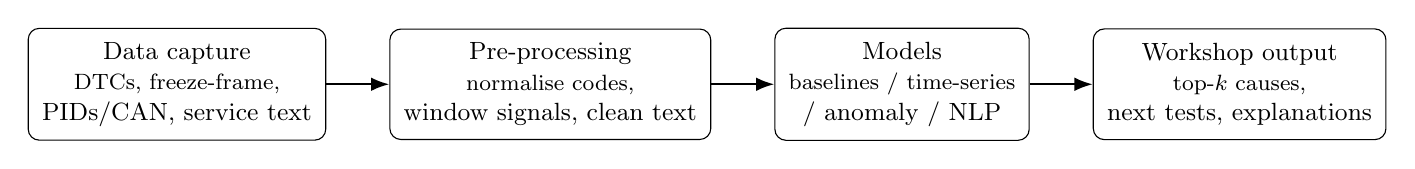
\begin{tikzpicture}[
  node distance=8mm and 8mm,
  box/.style={draw,rounded corners,align=center,inner sep=5pt,font=\small},
  arr/.style={-Latex,thick}
]
\node[box] (capture) {Data capture\\\footnotesize DTCs, freeze-frame,\\PIDs/CAN, service text};
\node[box, right=of capture] (prep) {Pre-processing\\\footnotesize normalise codes,\\window signals, clean text};
\node[box, right=of prep] (model) {Models\\\footnotesize baselines / time-series\\/ anomaly / NLP};
\node[box, right=of model] (output) {Workshop output\\\footnotesize top-$k$ causes,\\next tests, explanations};
\draw[arr] (capture) -- (prep);
\draw[arr] (prep) -- (model);
\draw[arr] (model) -- (output);
\end{tikzpicture}%
}
\caption{End-to-end pipeline for AI-assisted workshop diagnosis from heterogeneous evidence to technician-facing decision support.}\label{fig:pipeline}
\end{figure}

A crucial design choice is the definition of a \emph{case}. A case is often treated as a workshop visit, but visits can include multiple complaints and multiple interventions. In practice, many datasets are created by defining a case as ``one complaint-diagnosis-repair cycle'', which may require splitting a visit into multiple subcases.

\subsection{Problem formulation and labels}
Workshop learning problems are typically formulated around one of three targets:
\begin{itemize}
  \item \textbf{Fault category classification}: mapping each case to a fault family (e.g., misfire, air metering, wheel-speed sensor).
  \item \textbf{Root-cause component prediction/ranking}: mapping each case to a specific component or subsystem, and returning a top-$k$ shortlist.
  \item \textbf{Next-best test recommendation}: predicting which diagnostic test is most likely to reduce uncertainty, given the current evidence.
\end{itemize}

A common supervised formulation for component ranking is to learn a scoring function $s_m(x)$ for each component $m\in\{1,\dots,M\}$ given case evidence $x$ (DTCs, freeze-frame, time-series summaries, and optionally text), and convert scores to a distribution using a softmax:
\begin{equation}
  p(m\mid x) = \frac{\exp(s_m(x))}{\sum_{j=1}^{M} \exp(s_j(x))}.
\end{equation}

In workshop settings, ``ground truth'' is often noisy. A part replaced is not always the true root cause, and many visits end as ``no fault found'' \parencite{Hastie2009}. For this reason, root-cause \emph{ranking} is often a better formulation than top-1 prediction: it aligns with how technicians work (hypothesis generation and confirmation) and reduces the harm of overconfident single-output models \parencite{Molnar2022}.

\subsection{From raw logs to model-ready features}
The data pipeline usually includes:
\begin{enumerate}
  \item \textbf{DTC normalisation}: mapping generic and OEM codes into a consistent vocabulary; optionally adding hierarchical features (system/subsystem) and status bits.
  \item \textbf{Context normalisation}: retaining freeze-frame variables and derived context (cold start vs hot, steady vs transient).
  \item \textbf{Time-series windowing}: selecting segments that correspond to symptom reproduction, filtering out unrelated driving, and aligning multi-rate signals. In practice, window selection dominates model quality because models can otherwise learn driving-regime differences instead of fault signatures.
  \item \textbf{Text cleaning}: normalising abbreviations and spelling, removing personally identifiable information, and extracting symptom-action phrases (or using retrieval against historical cases).
\end{enumerate}

Rather than treating all fields equally, many deployments prioritise robust, low-variance features (DTCs + freeze-frame + a small set of engineered PID features) and then add time-series and text only when data quality is sufficient.

\subsection{Dataset challenges (data-centric view)}
The main limitations are data-centric \parencite{Hastie2009}.
\begin{itemize}
  \item \textbf{Label noise and ambiguity.} Repairs may be provisional, multiple parts may be replaced, and the recorded outcome may reflect business constraints rather than confirmed causality \parencite{Hastie2009}.
  \item \textbf{Class imbalance.} Common faults dominate frequency, while rare faults dominate cost and risk; this can lead to misleading accuracy if not addressed \parencite{Hastie2009}.
  \item \textbf{Variant shift.} Vehicle model year, engine variant, ECU software, and sensor suppliers change the mapping from symptoms to causes \parencite{Hastie2009}.
  \item \textbf{Missing and irregular signals.} Scan-tool logging is incomplete by design, and missingness can be informative (monitor unsupported) or accidental \parencite{SAEJ1979,ISO15031}.
\end{itemize}

\subsection{Evaluation protocol}
Evaluation should match the deployment scenario \parencite{Hastie2009}. Random record-level splits often leak vehicle identity and inflate performance \parencite{Hastie2009}. More realistic protocols split by vehicle (no VIN overlap), by time (train on earlier data, test on later), or by variant (hold out an ECU/engine family) \parencite{Hastie2009}.

For workshop decision support, predictive metrics should be complemented by workflow metrics such as top-$k$ hit rate. If the true component label for case $i$ is $y_i$ and the model returns a ranked shortlist $\pi_i(1),\dots,\pi_i(k)$, then:
\begin{equation}
  \mathrm{Hit}@k = \frac{1}{N}\sum_{i=1}^{N} \mathbf{1}\bigl[y_i \in \{\pi_i(1),\dots,\pi_i(k)\}\bigr].
\end{equation}

This should be reported alongside operational outcomes such as reduction in diagnostic time and reduction in unnecessary part replacement.

\section{AI Methods for Workshop Diagnosis}\label{sec:methods}

This section reviews model families that can be deployed in workshop decision support, organised by the dominant data modality. The emphasis is on practical pipelines: what the model consumes, what it outputs (classification vs ranking), and where failures typically occur.

\begin{figure}[t]
\raggedright
\resizebox{\linewidth}{!}{%
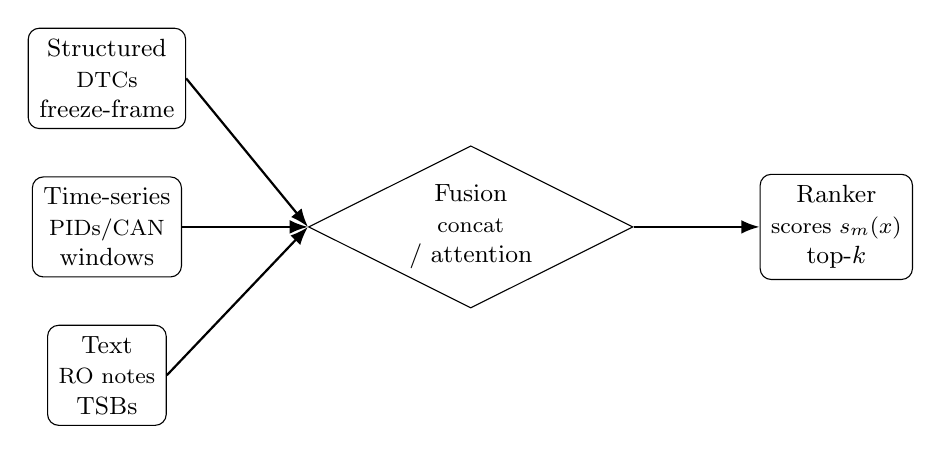
\begin{tikzpicture}[
  node distance=6mm and 8mm,
  box/.style={draw,rounded corners,align=center,inner sep=4pt,font=\small},
  fuse/.style={draw,diamond,aspect=2,align=center,inner sep=2pt,font=\small},
  arr/.style={-Latex,thick}
]
\node[box] (dtc) {Structured\\\footnotesize DTCs\\freeze-frame};
\node[box, below=of dtc] (ts) {Time-series\\\footnotesize PIDs/CAN\\windows};
\node[box, below=of ts] (txt) {Text\\\footnotesize RO notes\\TSBs};
\node[fuse, right=16mm of ts] (fusion) {Fusion\\\footnotesize concat\\/ attention};
\node[box, right=16mm of fusion] (rank) {Ranker\\\footnotesize scores $s_m(x)$\\top-$k$};
\draw[arr] (dtc.east) -- (fusion.west);
\draw[arr] (ts.east) -- (fusion.west);
\draw[arr] (txt.east) -- (fusion.west);
\draw[arr] (fusion.east) -- (rank.west);
\end{tikzpicture}%
}
\caption{Typical multimodal decision-support architecture: fuse structured diagnostics, time-series features, and text embeddings to produce a ranked shortlist of likely root causes.}
\label{fig:multimodal}
\end{figure}

\subsection{DTC- and freeze-frame-based baselines}
A strong starting point for workshop diagnosis is a baseline model trained on structured diagnostic artefacts: a multi-hot representation of DTCs, augmented with freeze-frame context. These models are attractive because they are robust to missingness, require minimal preprocessing, and align with the information technicians already use.
Typical implementations treat the task as (i) multi-label classification over fault categories or (ii) root-cause component ranking. Tree-based models (e.g.\@, gradient boosting) and regularised linear models are common because they can handle sparse inputs and provide some interpretability~\parencite{Friedman2001,Hastie2009}. In ranking mode, the model outputs calibrated probabilities or scores over components, with the technician consuming the top-$k$ shortlist.

The main failure mode is correlation without causality: DTC co-occurrence can arise from shared monitor enable conditions, not shared root cause. Adding freeze-frame variables (temperature, speed, load) and readiness status helps because it partially conditions on monitor context.

\subsection{Time-series modelling for sensor and CAN signals}
Time-series modelling aims to detect dynamic signatures that do not collapse into a single freeze-frame snapshot: oscillations, delays, drift, and intermittent behaviour. There are two dominant approaches.

\textbf{Feature-engineered pipelines} compute summary statistics (mean, variance, slope), frequency-domain features, and cross-signal relationships (e.g.\@, correlation between commanded and measured values). These features are then fed into classical predictors. Feature engineering is often data-efficient and easier to validate~\parencite{Hastie2009}.

\textbf{Representation learning pipelines} learn features directly from sequences. Recurrent networks such as LSTMs are a standard approach for temporal dependencies~\parencite{Hochreiter1997}, while attention-based encoders generalise to variable-length sequences and support flexible aggregation~\parencite{Vaswani2017}. In workshop contexts, these models must be trained with careful regime conditioning (idle vs cruise vs transient) to avoid learning driving-state differences.

A pragmatic hybrid strategy is common in industry: use deep encoders to generate embeddings from time-series windows, then use a simpler supervised model to map embeddings (plus DTC/freeze-frame features) to a ranked shortlist~\parencite{Friedman2001}.

\subsection{Anomaly detection for ``no-code'' faults}
Some of the most expensive workshop issues are ``no-code'' or intermittent faults where the vehicle does not reliably set a DTC\@. In these settings, anomaly detection can act as an early-warning or triage layer: learn what normal looks like for a given operating context and flag deviations~\parencite{Chandola2009}.

Autoencoder-based methods learn to reconstruct normal data and treat high reconstruction error as an anomaly score. Variational autoencoders (VAEs) provide a probabilistic version of this idea~\parencite{Kingma2014}. One-class embedding objectives (e.g.\@, deep one-class classification) aim to map normal observations into a compact region of representation space~\parencite{Ruff2018}.

The deployment challenge is controlling false alarms. ``Normal'' depends on ambient temperature, load, and vehicle variant; without explicit conditioning, anomaly detectors often learn regime differences rather than faults~\parencite{Chandola2009}.

\subsection{NLP on repair orders and service bulletins}
Text sources (repair orders, technician notes, and technical service bulletins) contain high-value information that is not present in sensor streams: symptom narratives (``stalls when hot''), constraints (``after rain''), and known fixes. NLP is therefore typically used in one of two ways.

\textbf{Extraction.} The goal is to convert noisy free text into structured fields: symptom entities, component mentions, and actions. In practice, this requires normalisation (abbreviations, misspellings) and de-identification~\parencite{Devlin2019}.

\textbf{Retrieval and case-based reasoning.} Rather than predicting a fix directly from text, a common strategy is to embed the current case and retrieve similar historical repairs \parencite{Manning2008}. Transformer encoders are widely used for text embeddings \parencite{Devlin2019}, but retrieval often performs better than end-to-end prediction when labelled data is limited. Retrieved cases provide a natural explanation: ``these past cases match your symptoms and were fixed by X''.

\subsection{Graph-based and causal approaches}
Purely correlational models can be brittle when symptoms are confounded by operating context or cascading failures. Graph-based approaches represent diagnostic knowledge explicitly as relationships among components, signals, and DTCs. This can be implemented as a knowledge graph for retrieval (paths from symptoms to components) or as a probabilistic graph model for inference \parencite{Pearl2009}.

Causal structure is particularly relevant because workshop diagnosis is intervention-rich: technicians perform tests, unplug sensors, swap components, or apply software updates \parencite{Pearl2009}. Models that treat tests as interventions can recommend the next-best test expected to reduce uncertainty, rather than only producing a most-likely fix. In practice, causal modelling is limited by the difficulty of obtaining clean intervention data at scale, but even lightweight graphs can improve robustness by constraining implausible hypotheses.

\subsection{Comparison summary}
Overall, workshop-ready systems tend to be hybrid. DTC/freeze-frame models provide strong, interpretable baselines; time-series models improve detection of intermittent and drift faults; NLP and retrieval connect evidence to historical fixes; and graph-based constraints can improve robustness. The main trade-off is between accuracy and maintainability: more complex multimodal systems can perform better but are harder to validate under domain shift.

\begin{table}[t]
\raggedright
\small
\caption{Summary of AI method families for workshop diagnosis and typical deployment trade-offs.}\label{tab:methods}
\begin{tabular}{p{0.18\linewidth} p{0.22\linewidth} p{0.22\linewidth} p{0.30\linewidth}}
\toprule
\textbf{Family} & \textbf{Inputs} & \textbf{Output} & \textbf{Strengths / failure modes}\\
\midrule
DTC + freeze-frame baselines & DTC set, status bits, freeze-frame PIDs & Fault class or top-$k$ causes & Robust and cheap; can learn spurious co-occurrence unless conditioned on context.\\
Time-series models & PID/CAN windows (optionally with context) & Class/rank/anomaly score & Captures dynamics and intermittent faults; sensitive to regime shift and window selection.\\
Anomaly detection & ``Normal'' logs by regime/variant & Anomaly score + deferral & Useful for no-code faults; false alarms if conditioning is weak.\\
Text/NLP + retrieval & Repair orders, notes, TSBs & Similar-case retrieval + suggested fixes & Strong explainability; brittle if vocabulary/abbreviations drift and labels are weak.\\
Graph/causal constraints & Component/signal graph + observed evidence & Constrained ranking + next tests & Improves robustness and test planning; limited by available intervention data.\\
\bottomrule
\end{tabular}
\end{table}

\section{Limitations, Safety, and Evaluation}
Section \ref{sec:methods} emphasised that workshop AI is primarily a decision-support technology. This section focuses on the practical limits that determine whether a system is safe, trustworthy, and worth deploying.

\subsection{Evaluation metrics and baselines}
Workshop evaluation should include both predictive metrics and workflow metrics.

\textbf{Predictive metrics.} For root-cause ranking, top-$k$ hit rate (\Cref{sec:data}) is typically more informative than top-1 accuracy because it matches how technicians use recommendations. For imbalanced fault classification, precision--recall curves are often more appropriate than ROC curves. For anomaly detection, evaluation should report false-alarm rates under defined operating regimes \parencite{Hastie2009,QuioneroCandela2009}.

\textbf{Workflow metrics.} The most deployment-relevant measures include reduction in time-to-diagnosis, reduction in repeat visits, reduction in unnecessary part replacement, and improvement in first-time-fix rate. These metrics require either controlled trials (ideal) or careful retrospective studies that avoid hindsight bias.

\textbf{Baselines.} Any AI system should be compared to at least (i) code-lookup heuristics (e.g.\@, most common fix per DTC), (ii) technician-guided diagnostic procedures, and (iii) simple ML baselines trained only on DTC/freeze-frame features.

\subsection{Uncertainty calibration and deferral}
In workshop decision support, abstention is a core safety mechanism. When a model is uncertain---for example, because the case is out-of-distribution or evidence is contradictory---it should defer to manual testing rather than outputting a misleading top-1 recommendation.

Operationally, this can be implemented with calibrated confidence thresholds, where the system produces a shortlist only if its predicted confidence exceeds a target level. Calibration matters because raw neural scores are often overconfident \parencite{Guo2017}. Uncertainty should also be surfaced to the user interface: a low-confidence output should trigger recommendations for additional evidence capture rather than a direct repair action.

\subsection{Robustness and domain shift}
Domain shift is the default condition in automotive diagnosis: model year changes, calibration updates, and sensor supplier variation all alter signal distributions. Robustness practices therefore need to be built into the lifecycle.
\begin{itemize}
  \item \textbf{Split design.} Validation should hold out vehicles and, where possible, entire variants.
  \item \textbf{Drift monitoring.} Deployed models should monitor input distributions and error proxies to detect drift.
  \item \textbf{Versioning and rollback.} Models must be versioned with the ability to roll back when performance degrades.
\end{itemize}

Without these controls, models may appear accurate in development but fail silently in deployment.

\subsection{Cybersecurity and adversarial considerations}
Connected diagnostics and richer logging increase the attack surface. If diagnostic recommendations influence repairs, warranty decisions, or software updates, adversaries may have incentives to manipulate evidence. Even without explicit ``adversarial ML'', practical threats include:
\begin{itemize}
  \item spoofed sensor readings or injected CAN messages during logging;
  \item tampering with logs at rest or in transit;
  \item data poisoning in shared or federated learning settings.
\end{itemize}

Mitigations include authenticated logging, access control, integrity checks, and separating advisory output from safety-critical control decisions \parencite{Bosch1991,ISO14229}.

\subsection{Safety and accountability}
AI diagnosis should be deployed with clear accountability: the system recommends, but the technician remains responsible for the final repair decision. For safety and warranty contexts, audit trails should record what evidence was used, what the model recommended, and what action was taken.

Explainability supports accountability. It should not be treated as an afterthought: systems need to provide justifications (relevant signals, retrieved similar cases, or ruled-out hypotheses) that allow technicians to challenge outputs and avoid automation bias \parencite{Molnar2022}.

\subsection{Deployment recommendations (practical checklist)}
To translate model performance into workshop value, deployments should:
\begin{itemize}
  \item define a minimum evidence set per case (DTCs + freeze-frame + a small PID panel) and ensure consistent capture;
  \item validate under realistic splits (by vehicle/variant and time) and monitor post-deployment drift;
  \item use calibrated uncertainty with abstention, surfacing ``collect more evidence'' actions when confidence is low;
  \item provide technician-facing explanations (top-$k$ list + key signals + suggested next test) to reduce automation bias.
\end{itemize}

\section{Conclusion}

\subsection{Summary of findings}
This paper reviewed how AI methods are applied to workshop diagnosis using DTCs, freeze-frame context, time-series sensor evidence, and service text. Across approaches, the most practical near-term capability is not fully automated diagnosis but decision support that ranks likely causes, surfaces relevant historical knowledge, and guides technicians toward high-value tests.

\subsection{Implications for workshop diagnosis}
AI-enabled triage can reduce diagnostic time and unnecessary part replacement when it is built on robust data pipelines, validated under variant shift, and deployed with calibrated uncertainty and explanations. The implication is that organisations should treat AI diagnosis as an operational system---data capture, monitoring, and governance---rather than a one-off model training exercise.

\subsection{Key research gaps}
Key gaps remain in (i) benchmark datasets that reflect real workshop constraints, (ii) methods robust to noisy repair labels and ambiguous outcomes, (iii) multimodal fusion that respects operating context, and (iv) assurance methods for safety-aware deployment under domain shift. Closing these gaps is likely to determine whether AI diagnosis becomes routine workshop infrastructure over the next decade.

\newpage
\phantomsection
\addcontentsline{toc}{section}{References}
\printbibliography

\end{document}